% sample.tex
\documentclass[9pt]{beamer}
\usepackage{pdfpages}
\usepackage{hyperref}
\usepackage[capitalise,nameinlink]{cleveref}
\hypersetup{colorlinks=true, linkcolor=blue, citecolor=blue, urlcolor=blue}
\usepackage{booktabs}
\definecolor{darkblue}{rgb}{0.0, 0.0, 0.55}
\usepackage{multicol}
\usepackage{xcolor}
\usepackage{pbox}
\usepackage{color}
\colorlet{linkequation}{blue}
\usepackage{bm, bbm}
\definecolor{forestgreen(web)}{rgb}{0.13, 0.55, 0.13}
\usepackage{float}
\usepackage{soul}
% \usepackage{hyperref}
% \usepackage[capitalise,nameinlink]{cleveref}
\usepackage[round]{natbib}
\usepackage{subfig}
% \captionsetup[subfigure]{labelformat=empty}  % Commented out as it's unused
\usepackage{algorithm,algorithmic}
\renewcommand{\algorithmicrequire}{\textbf{Input:}}
\renewcommand{\algorithmicensure}{\textbf{Output:}}
\usepackage{graphicx}
\usepackage{subcaption} 
\usepackage{mathtools}
\usepackage{multicol}
\usepackage{pgf,tikz}
\usepackage[round]{natbib}
\usepackage{makecell}

% \usepackage{fontspec}
% \usepackage{xeCJK}
% \xeCJKsetup{CJKmath=false}
% \setCJKmainfont{SimSun}
\bibliographystyle{plainnat}

\usetikzlibrary{arrows,shapes.arrows,shapes.geometric,shapes.multipart,fit,automata,decorations.pathmorphing,positioning}
\tikzset{
	%Define standard arrow tip
	>=stealth',
	%Define style for boxes
	true/.style={
		rectangle,
		draw=black, very thick,
		text width=6.5em,
		minimum height=2em,
		text centered,
		fill=gray, opacity = 0.5},
	punkt/.style={
		rectangle,
		rounded corners,
		draw=black, very thick,
		text width=6.5em,
		minimum height=2em,
		text centered},
	est/.style={
		circle,
		draw=black, very thick,
		text centered},
	shade/.style={
		circle,
		draw=black, very thick, fill=gray!50,
		text centered},
	weight/.style={
		circle,
		draw=black, very thick,
		text width=6.5em,
		minimum height=2em,
		text centered},
	% Define arrow style
	pil/.style={
		->,
		thick,
		shorten <=2pt,
		shorten >=2pt,},
	double/.style={
		<->,
		thick,
		shorten <=2pt,
		shorten >=2pt,},
	dash/.style={
		dashed,
		thick,
		shorten <=2pt,
		shorten >=2pt,},
	dashdouble/.style={
		<->,
		dashed,
		thick,
		shorten <=2pt,
		shorten >=2pt,}
}
%gets rid of footer
%will override 'frame number' instruction above
%comment out to revert to previous/default definitions
\setbeamertemplate{footline}{}
\usepackage{listings}
\definecolor{turquoise}{rgb}{0.19, 0.84, 0.78}

\definecolor{codegreen}{rgb}{0,0.6,0}
\definecolor{codegray}{rgb}{0.5,0.5,0.5}
\definecolor{codepurple}{rgb}{0.58,0,0.82}
\definecolor{backcolour}{rgb}{0.95,0.95,0.92}

\lstdefinestyle{mystyle}{
    backgroundcolor=\color{backcolour},    
    commentstyle=\color{codegreen},
    keywordstyle=\color{magenta},
    numberstyle=\tiny\color{codegray},
    stringstyle=\color{codepurple},
    basicstyle=\ttfamily\footnotesize,
    breakatwhitespace=false,         
    breaklines=true,                 
    captionpos=b,                    
    keepspaces=true,                 
    numbers=left,                    
    numbersep=5pt,                  
    showspaces=false,                
    showstringspaces=false,
    showtabs=false,                  
    tabsize=2
}

\lstset{style=mystyle}
\usepackage[most]{tcolorbox}
%\usetheme{default}
\usepackage{amsmath}
\usepackage{amsthm}
\usepackage{amsfonts}
\usepackage{amsopn}
\usepackage{scalerel}

% Define argmin operator
\DeclareMathOperator*{\argmin}{arg\,min}

\newcommand\Wider[2][7.5em]{%
\makebox[\linewidth][c]{%
  \begin{minipage}{\dimexpr\textwidth+#1\relax}
  \raggedright#2
  \end{minipage}%
  }%
}
\newcommand\reallywidehat[1]{%
\begin{array}{c}
\stretchto{
  \scaleto{
    \scalerel*[\widthof{#1}]{\bigwedge}
    {\rule[-\textheight/2]{1ex}{\textheight}} %WIDTH-LIMITED BIG WEDGE
  }{1.25\textheight} % THIS STRETCHES THE WEDGE A LITTLE EXTRA WIDE
}{0.5ex}\\           % THIS SQUEEZES THE WEDGE TO 0.5ex HEIGHT
#1\\                 % THIS STACKS THE WEDGE ATOP THE ARGUMENT
\rule{-1ex}{0ex}
\end{array}
}
\usepackage{bbm}
% amssymb package, useful for mathematical symbols
\usepackage{amssymb}
\setbeamertemplate{theorems}[numbered]
\setbeamertemplate{lemma}[numbered]
\setbeamertemplate{corollary}[numbered]

\newcommand{\calW}{{\mathcal{W}}}
\def\m{\mathrm{m}}
\def\bbE{\mathbb{E}}
\def\bbP{\mathbb{P}}
\def\E{\mathsf{E}}
\def\Holder{\text{H\"{o}lder}}
\def\Pr{\mathsf{Pr}}
\def\EIF{\mathsf{EIF}}
\def\NIF{\mathsf{NIF}}
\def\bias{\texttt{bias}}
\def\var{\texttt{var}}
\def\cov{\texttt{cov}}

\def\tilde{\widetilde}
\def\P{\mathsf{P}}
\def\calP{\mathcal{P}}
\def\d{\mathrm{d}}
\def\calG{\mathcal{G}}
\def\pa{\mathsf{pa}}
\def\ch{\mathsf{ch}}
\def\an{\mathsf{an}}
\def\de{\mathsf{de}}
\def\bV{\bm{V}}
\def\bv{\bm{v}}
\def\be{\bm{e}}
\def\var{\mathsf{var}}
\def\cov{\mathsf{cov}}
\def\df{\mathrm{df}}
\def\init{\mathrm{init}}
\def\t{\mathrm{t}}

\DeclareRobustCommand{\stred}[1]{{\sethlcolor{cyan}\st{#1}}}
\setbeamercovered{transparent}
\setbeamertemplate{theorems}[numbered]
\makeatletter
\def\th@mystyle{%
    \normalfont % body font
    \setbeamercolor{block title example}{bg=gray,fg=white}
    \setbeamercolor{block body example}{bg=white,fg=black}
    \def\inserttheoremblockenv{exampleblock}
  }
\makeatother
\theoremstyle{mystyle}
\definecolor{dblue}{named}{fg}
\newtheorem{mytheorem}{Theorem}
\newtheorem{mycorollary}{Corollary}
\newtheorem{myprop}{Proposition}
\newtheorem{mylemma}{Lemma}
\newtheorem{myfact}{Fact}
\newtheorem{mydefn}{Definition}
\newtheorem{myeg}{Example}
\newtheorem{myremark}{Remark}
\newtheorem{myqn}{Qn}
\definecolor{ForestGreen}{RGB}{34,139,34}

\makeatletter
\def\th@mystyletwo{%
    \normalfont % body font
    % \setbeamercolor{block title example}{bg=orange,fg=white}
    \setbeamercolor{block body example}{bg=orange!20,fg=black}
    \def\inserttheoremblockenv{exampleblock}
  }
\makeatother
\theoremstyle{mystyletwo}
\newtheorem*{myblock}{}
\usepackage{tikzsymbols}
\usepackage{textcomp}

\definecolor{greyone}{RGB}{77,77,77}
\setbeamercolor{palette quaternary}{fg=white}
\setbeamercolor{titlelike}{parent=palette quaternary}
% \usepackage{enumitem}
\setbeamercolor{title}{fg=black}
\setbeamerfont{title}{series=\bf, size=\Large}
\setbeamercolor{frametitle}{fg=brown!150}

\setbeamerfont{frametitle}{size=\Large}
\setbeamertemplate{itemize/enumerate body begin}{\normalsize}
\setbeamertemplate{itemize/enumerate subbody begin}{\normalsize}

%gets rid of bottom navigation bars
%\setbeamertemplate{footline}[frame number]{}

\setbeamertemplate{frametitle}[default][center]

%gets rid of bottom navigation symbols
\setbeamertemplate{navigation symbols}{}

\newcommand\independent{\protect\mathpalette{\protect\independenT}{\perp}}
\def\independenT#1#2{\mathrel{\rlap{$#1#2$}\mkern2mu{#1#2}}}

%\expandafter\def\expandafter\insertshorttitle\expandafter{%
%  \insertshorttitle\hfill%
%  \insertframenumber\,/\,\inserttotalframenumber}
\addtobeamertemplate{navigation symbols}{}{ \hspace{1em}    \usebeamerfont{footline}%
    \large\insertframenumber / \inserttotalframenumber }

\def\calF{\mathcal{F}}
\def\Holder{H\"{o}lder}
\def\bbE{\mathbb{E}}
\def\bE{\mathbf{E}}
\def\bZ{\mathbf{Z}}
\def\bz{\mathbf{z}}
\def\bX{\mathbf{X}}
\def\bx{\mathbf{x}}
\def\bY{\mathbf{Y}}
\def\y{\mathrm{y}}
\def\a{\mathrm{a}}
\def\bbP{\mathbb{P}}
\def\Infl{\mathsf{IF}}
\def\diff{\mathrm{d}}
\def\a{\mathrm{a}}
\def\b{\mathrm{b}}
\def\hata{{\color{blue}\hat{\a}}}
\def\hatb{{\color{blue}\hat{\b}}}
\def\N{\mathrm{N}}
\def\bmu{\bm{\mu}}
\def\bSigma{\bm{\Sigma}}
\def\bbeta{\bm{\beta}}
\def\balpha{\bm{\alpha}}
\def\db{\mathsf{db}}
\def\reg{\mathsf{reg}}
\def\bI{\mathbf{I}}

\def\bbX{\mathbb{X}}

% Custom block width commands
\newcommand{\fullwidth}{\linewidth}
\newcommand{\halfwidth}{0.49\linewidth}
\newcommand{\thirdwidth}{0.32\linewidth}
\newcommand{\unknowna}[1]{\textcolor{teal!70!black}{#1}}
\newcommand{\unknownb}[1]{\textcolor{orange!80!black}{#1}}
\newcommand{\unknownc}[1]{\textcolor{violet!70!black}{#1}}
\newcommand{\unknownd}[1]{\textcolor{gray!60!black}{#1}}
\newcommand{\unknowne}[1]{\textcolor{green!60!black}{#1}}
\newcommand{\unknownh}[1]{\textcolor{blue!65!black}{#1}}



\def\f{\mathrm{f}}

\def\bbE{\mathbb{E}}
\def\bbP{\mathbb{P}}
\def\E{\mathsf{E}}
\def\Holder{\text{H\"{o}lder}}
\def\Pr{\mathsf{Pr}}
\def\EIF{\mathsf{EIF}}
\def\NIF{\mathsf{NIF}}
\def\bias{\texttt{bias}}
\def\var{\texttt{var}}
\def\cov{\texttt{cov}}
\def\hat{\widehat}
\def\tilde{\widetilde}
\def\P{\mathsf{P}}
\def\calP{\mathcal{P}}
\def\d{\mathrm{d}}
\def\calG{\mathcal{G}}
\def\pa{\mathsf{pa}}
\def\ch{\mathsf{ch}}
\def\an{\mathsf{an}}
\def\de{\mathsf{de}}
\def\bV{\bm{V}}
\def\bv{\bm{v}}
\def\be{\bm{e}}
\def\bU{\bm{U}}
\def\var{\mathsf{var}}
\def\cov{\mathsf{cov}}
\def\df{\mathrm{df}}
\def\init{\mathrm{init}}
\def\t{\mathrm{t}}
\newcommand{\calX}{{\mathcal{X}}}
\newcommand{\bbU}{{\mathbb{U}}}
\newcommand{\bbV}{{\mathbb{V}}}

\def\calF{\mathcal{F}}
\def\Holder{H\"{o}lder}
\def\bbE{\mathbb{E}}
\def\bE{\mathbf{E}}
\def\bZ{\mathbf{Z}}
\def\bX{\mathbf{X}}
\def\bx{\mathbf{x}}
\def\bY{\mathbf{Y}}
\def\A{\mathrm{A}}
\def\Y{\mathrm{Y}}
\def\y{\mathrm{y}}
\def\a{\mathrm{a}}
\def\bbP{\mathbb{P}}
\def\Infl{\mathsf{IF}}
\def\diff{\mathrm{d}}
\def\a{\mathrm{a}}
\def\b{\mathrm{b}}
\def\hata{{\color{blue}\hat{\a}}}
\def\hatb{{\color{blue}\hat{\b}}}
\def\N{\mathrm{N}}

\def\bmu{\bm{\mu}}

\def\bbeta{\bm{\beta}}
\def\balpha{\bm{\alpha}}
\def\db{\mathsf{db}}
\def\reg{\mathsf{reg}}
\def\bI{\mathbf{I}}

\def\({\left(}
\def\){\right)}
\def\[{\left[}
\def\]{\right]}
\def\bbR{\mathbb{R}}

\def\f{\mathrm{f}}
\def\({\left(}
\def\){\right)}
\def\[{\left[}
\def\]{\right]}
\def\bbR{\mathbb{R}}
    
\tcbset{
  mytheoremstyle/.style={
    colback=white,
    colframe=blue!60!black,
    fonttitle=\bfseries,
    coltitle=black,
    title={Questions},
    sharp corners,
    boxrule=0.8pt,
    left=6pt, right=6pt, top=6pt, bottom=6pt,
  }
}
\tcbset{
  myposterstyle/.style={
    colback=white,
    colframe=blue!80!black,
    coltitle=white,
    colbacktitle=blue!80!black,
    fonttitle=\bfseries,
    boxrule=1pt,
    sharp corners,
    enhanced,
    left=6pt, right=6pt, top=6pt, bottom=6pt,
    titlerule=0mm,
    toptitle=1mm,
    bottomtitle=1mm
  }
}

% user-defined commands
% user-defined macros
\newcommand{\pdfu}{\texorpdfstring{$U$}{U}}
\newcommand{\pdfv}{\texorpdfstring{$V$}{V}}
\newcommand{\libref}[2]{\href{#2}{\texttt{#1}}}

\newcommand{\mobius}{M\"obius}

\newcommand{\numpy}{\libref{numpy}{https://numpy.org/}}
\newcommand{\torch}{\libref{pytorch}{https://pytorch.org/}}

% simplified command
\newcommand{\wt}{\overline}
\newcommand{\diag}{\mathsf{Diag}}
\newcommand{\diagp}[1]{\diag(#1)}
\newcommand{\sPi}{\pi}
\newcommand{\sper}{\sigma}

% HOIF
\newcommand{\IF}{\mathbb{IF}}
\newcommand{\BD}{\mathbb{BD}}
\newcommand{\factorial}[1]{#1\mathpunct{!}}

% stats notations
\newcommand{\uset}{\calU}
\newcommand{\usetnm}[2]{\uset\left(#1,#2\right)}
\newcommand{\vset}{\calV}
\newcommand{\vsetp}[2]{\vset(#1,#2)}

\newcommand{\ustat}{\mathbb{U}}
\newcommand{\vstat}{\mathbb{V}}
\newcommand{\ustatp}[2]{\ustat(#1,#2)}
\newcommand{\vstatp}[2]{\vstat(#1,#2)}

% set notations
\newcommand{\samplespace}{\bbX}
\newcommand{\takesetp}[1]{\mathsf{set}[#1]}
\newcommand{\cartesianprod}{\bigotimes}

% combinatoric notations
\newcommand{\perm}[1]{\mathsf{Perm}(#1)}
\newcommand{\partition}{\Pi}

\newcommand{\partitionp}[1]{\partition_{#1}}
\newcommand{\finest}{\mathsf{Fin}}
\newcommand{\finestp}[1]{\finest[#1]}
\newcommand{\coarsest}{\mathsf{Coa}}
\newcommand{\coarsestp}[1]{\coarsest[#1]}
\newcommand{\cover}{\mathcal{C}}
\newcommand{\stirling}{\calS}
\newcommand{\stirlingp}[2]{\stirling(#1,#2)}

% tensor notations
\newcommand{\ndim}{\mathsf{ndim}}
\newcommand{\ndimp}[1]{\ndim(#1)}
\newcommand{\rank}{\mathrm{rank}}
% \newcommand{\dim}{\mathrm{dim}}
\newcommand{\dimp}[2]{\dim[#1](#2)}
\newcommand{\indexset}{\mathsf{Indices}}
\newcommand{\teq}{\overset{\mathrm{t.e.}}{=}}
\newcommand{\canonicalform}{\mathsf{canonical}}
\newcommand{\tensorcontraction}{\mathsf{Contraction}}

% partial order in partition
\newcommand{\pleq}{_\preceq}
\newcommand{\pgeq}{\succeq}
\newcommand{\pless}{\prec}
\newcommand{\pgreater}{\succ}

% Graph notations
\newcommand{\degp}[2]{\deg_{#2}(#1)}
\newcommand{\vertices}[0]{V}
\newcommand{\verticesp}[1]{V(#1)}
\newcommand{\edges}[0]{E}
\newcommand{\edgesp}[1]{E(#1)}
\newcommand{\neighborvg}[2]{N_{#2}(#1)}

\newcommand{\treewidth}{\mathsf{tw}}
\newcommand{\treewidthp}[1]{\mathsf{tw}(#1)}
\newcommand{\quotientgraphp}[1]{\mathcal{Q}(#1)}
\newcommand{\graphset}{\mathcal{G}^{*}}
\newcommand{\graphsetne}[2]{\mathcal{G}_{#1,#2}^{*}}

\newcommand{\degeneracy}{D}
\newcommand{\degeneracyg}[1]{\degeneracy(#1)}
\newcommand{\completegraphp}[1]{\mathrm{K}_{#1}}
\newcommand{\graphtype}[1]{G_{#1}}
\newcommand{\motifrg}[2]{\mathsf{C}(#1,#2)}
% Oh-notaions
\newcommand{\greater}{\Omega}
\newcommand{\less}{O}
\newcommand{\muchgreater}{\omega}
\newcommand{\muchless}{o}
\newcommand{\appequal}{\Theta}

% operators
\newcommand{\eliminatevg}[2]{\mathsf{elim}_{#1}(#2)}


\def\eps{\epsilon}
\def\veps{\varepsilon}
\def\mse{\mathsf{mse}}

% code libs 
\def\package{\libref{u-stats}{https://github.com/Amedar-Asterisk/U-Statistics-python}}

\newcommand{\numpyeinsum}{\libref{numpy.einsum}{https://numpy.org/doc/2.1/reference/generated/numpy.einsum.html}}

\newcommand{\torcheinsum}{\libref{pytorch.einsum}{https://pytorch.org/docs/stable/generated/torch.einsum.html}}
\newcommand{\opteinsum}{\libref{opt-einsum}{https://dgasmith.github.io/opt_einsum/}}
\newcommand{\igraph}{\libref{igraph}{https://igraph.org/}}
\graphicspath{{Figures_slides/}}

\title{On Computing and the Complexity of Computing a Class of Higher-Order U/V-Statistics, Exactly}
\date{July 27, 2025}
\author[Ruiqi Zhang]{Ruiqi Zhang\\
School of Mathematical Sciences, East China Normal University\\
Shanghai, China \\
Email: \texttt{zrq1706@outlook.com} \\
}


\begin{document}
\begin{frame}
    \maketitle
\end{frame}

\begin{frame}
  \frametitle{Coauthors}
  \centering
  \begin{minipage}[b]{0.4\textwidth}
    \centering
    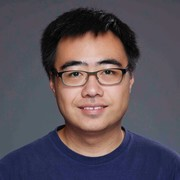
\includegraphics[height=4cm]{Figures_slides/Lin_Liu.png}
    Lin Liu, Assistant Professor @SJTU
  \end{minipage}
  \hfill
  \begin{minipage}[b]{0.4\textwidth}
    \centering
    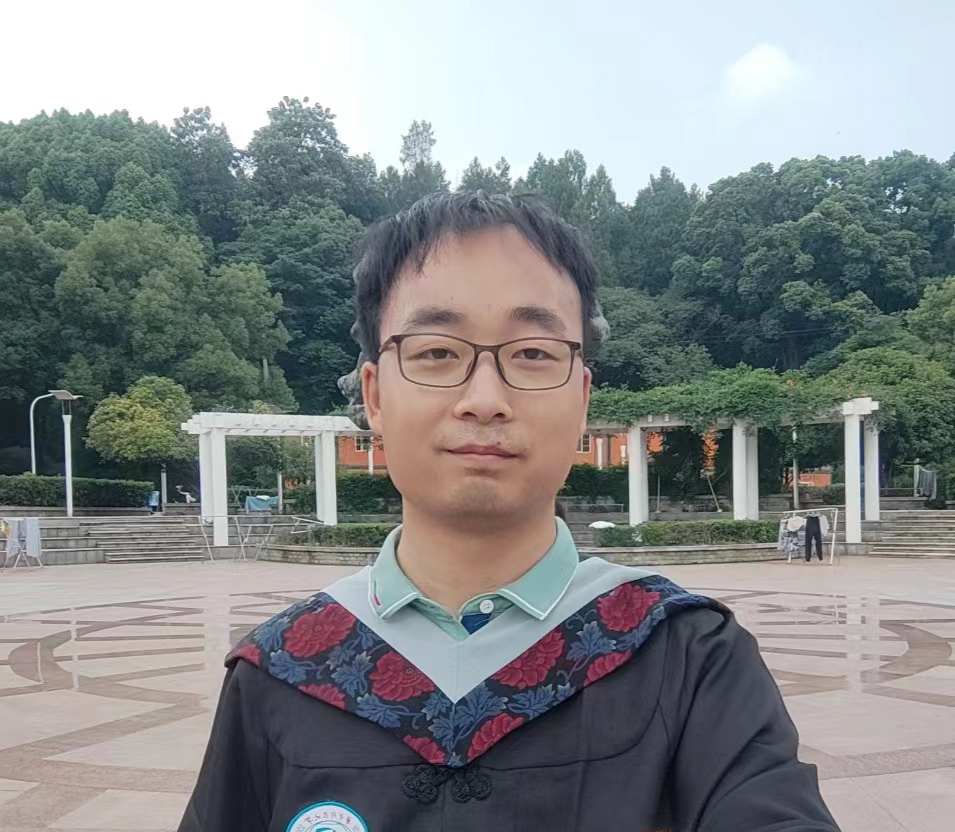
\includegraphics[height=4cm]{Figures_slides/Xingyu_Chen.jpg}
    Xingyu Chen, 2nd-year PhD student @SJTU
  \end{minipage}
\end{frame}


% \begin{frame}\frametitle{Outline}
%     \tableofcontents[currentsection, sectionstyle=show, subsectionstyle=show]
% \end{frame}

\section{Introduction}
\begin{frame}
    \frametitle{Outline}
    \tableofcontents[currentsection, sectionstyle=show/shaded, subsectionstyle=show/shaded/shaded]
\end{frame}
\begin{frame}
    \frametitle{U/V-Statistics}
    U-statistics are generally used to construct unbiased estimators of population parameters.
    \begin{itemize}
        \item Given a kernel $h(x_1, \ldots, x_m): \calX^m \to \bbR$ and a sequence of samples $X_1, \ldots, X_n$. 
        \item The U-statistic takes the form
              \begin{align*}
                  U_{n,m}[h] = \sum_{i_1 \neq i_2 \neq \cdots \neq i_m} h(X_{i_1}, \ldots, X_{i_m}).
              \end{align*}
        \item The V-statistic takes the form
              \begin{align*}
                  V_{n,m}[h] = \sum_{i_1 = 1}^{n} \cdots \sum_{i_m = 1}^{n} h(X_{i_1}, \ldots, X_{i_m}).
              \end{align*}
        \item We focus on high-order U/V-statistics ($m \geq 3$) especially U-statistics.
    \end{itemize}
\end{frame}

\begin{frame}
    \frametitle{Example 1: U-Statistics in Causal Inference: HOIFs}
    \begin{itemize}
        \item Higher-order influence functions (HOIFs) \citep{robins2008higher, robins2016technical} are rate-optimal estimators for many causal parameters. 
        % under various structural assumptions (smoothness, structure-agnostic, …)
        \item HOIF is a high order U-statistic, whose order can up to $m \sim \sqrt{\log n}$.
        \item Efficient algorithms are needed to compute these statistics in practice.
        \begin{itemize}
            \item $n=100, m=4: {\color{red} \text{more than } 200s}$.
        \end{itemize}
        \item For example, HOIF of the treatment-specific mean reads as
              \begin{align*}
                  \hat{\tau}_{m} = \sum_{j = 2}^{m} (-1)^{j} \ustat_{n,j}[h^{(j)}],
              \end{align*}
              where
              \begin{align*}
                  h^{(j)}(O_{i_1}, \ldots, O_{i_j}) = & a_{i_{1}} \phi (Z_{i_{1}})^{\top} (\phi(Z_{i_2})\phi(Z_{i_3})^\top - \mathbb{I}) \\
                & \cdots (\phi(Z_{i_{j-2}})\phi(Z_{i_{j-1}})^\top - \mathbb{I}) \phi(Z_{i_j})b_{i_j}, 
              \end{align*}
              which is the combination of functions like
              \begin{align*}
                  h^{(j)}_k(O_{i_1}, \ldots, O_{i_k}) = a_{i_{1}} \phi (Z_{i_{1}})^{\top} \phi(Z_{i_2}) \cdots \phi(Z_{i_{k-1}})^\top \phi(Z_{i_k})b_{i_k}. 
              \end{align*}
    \end{itemize}
\end{frame}

\begin{frame}
    \frametitle{Example 2: Dependence Measures}
    \begin{itemize}
        \item High-order U-statistics are also used to estimate dependence measures, such as Distance Covariance ($\mathsf{dCov}^2$) \citep{szekely2007measuring}.
        \item $\mathsf{dCov}^2$ can be represented as a 4-th order U-statistic \citep{yao2018testing}:
              \begin{align*}
                  \mathsf{dCov}^2(X, Y) = \frac{(n-4)!}{n!} \sum_{i \neq j \neq q \neq r}
                  a_{i,j}b_{q,r} + a_{i,j}b_{i,j} - a_{i,j}b_{i,q} - a_{i,j}b_{j,r}
              \end{align*}
              where $a_{i,j} = \|X_i-X_j\|_2$ and $b_{i,j} = \|Y_i-Y_j\|_2$.
        \item It costs {\color{red} $3787.84$s} to compute $\mathsf{dCov}^2$ on the S\&P 500 historical data according to \cite{shao2025u}. 
        \begin{itemize}
            \item This motivates them to use randomized incomplete U-statistic instead. 
        \end{itemize}
    \end{itemize}
\end{frame}


\begin{frame}
\frametitle{Example 3: Motif Counts}
\begin{itemize}
    \item Motif counts refer to the number of occurrences of small subgraphs (motifs) in a random graph. 
    \item They can be used to test certain properties of the underlying random graphon \citep{chatterjee2024higher}.
    \item Such as 3-node motifs,
        \begin{figure}
          \centering
          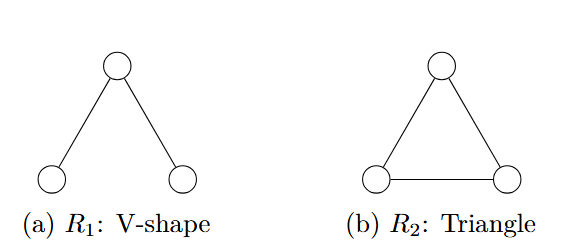
\includegraphics[width=0.5\linewidth]{motif3.jpg}
          \caption*{3-node motifs in a random graph}
          \label{fig:motif3}
      \end{figure}
\end{itemize}
\end{frame}

\begin{frame}
\frametitle{Example 3: Motif Counts}
\begin{itemize}
    \item And 4-node motifs, 
        \begin{figure}
          \centering
          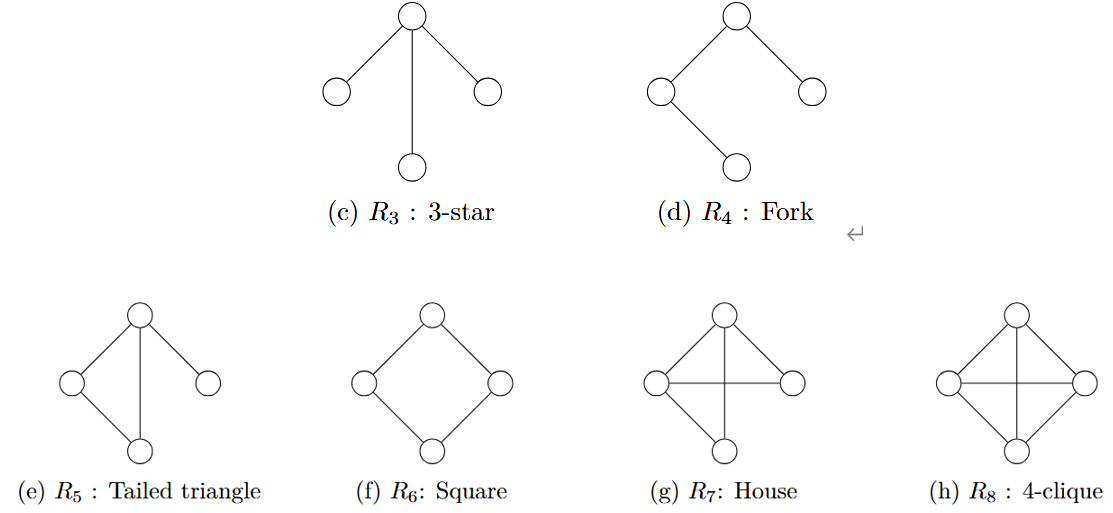
\includegraphics[width=0.9\linewidth]{motif4.jpg}
          \caption*{4-node motifs in a random graph}
          \label{fig:motif4}
        \end{figure}
\end{itemize}
\end{frame}

\begin{frame}
\frametitle{Example 3: Motif Counts}
\begin{itemize}
    \item The motif counts can also be written as a form similar to U-statistics. 
    \item For example, the 3-node motif counts can be written as
    \begin{itemize}
        \item V-shape:
        \begin{align*}
                C(R_1) = \frac{1}{2} \sum_{ i_1 \neq i_2 \neq i_3}  A_{i_1, i_2} A_{i_2, i_3}  B_{i_3, i_1}
        \end{align*}
        \item Triangle:
        \begin{align*}
                C(R_2) = \frac{1}{6} \sum_{ i_1 \neq i_2 \neq i_3}  A_{i_1, i_2} A_{i_2, i_3}  A_{i_3, i_1}
        \end{align*}
        \item $A$ is the adjacency matrix of a graph and $B = 1 -A$ is the complement of $A$.
    \end{itemize}
    \item Counting 4-node motifs may cost {\color{red} more than $6 \times 10^4$s}.  
\end{itemize}
\begin{figure}
          \centering
          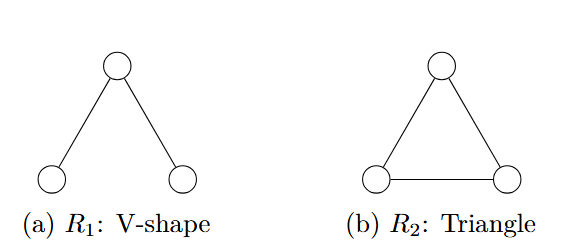
\includegraphics[width=0.4\linewidth]{motif3.jpg}
          \caption*{3-node motifs in a random graph.}
          \label{fig:motif3}
\end{figure}
\end{frame}

% \begin{frame}
% \frametitle{More Examples}
% \begin{itemize}
%     \item \cite{} used U-statistics to
%     \item \cite{} used U-statistics to
% \end{itemize}
% \end{frame}

\section{On Computing U/V-Statistics}
\begin{frame}
    \frametitle{Outline}
    \tableofcontents[currentsection, sectionstyle=show/shaded, subsectionstyle=show/shaded/shaded]
\end{frame}

\begin{frame}
    \frametitle{Difficulties in Computing U/V-Statistics}
    Difficulties:
    \begin{itemize}
        \item Computational Complexity: $O(n^m)$
              \begin{itemize}
                  % \item evaluate the kernel on $O(n^m)$ groups of arguments
                  \item $O(n^m)$ summands
              \end{itemize}
        \item Lack of using high-efficient computing techniques such matrix operation, tensor operation, etc.
              \begin{itemize}
                  \item Existing implementations are (to our knowledge) all based on for-loops.
              \end{itemize}
    \end{itemize}
    The following questions naturally arise:
    \begin{block}{Question 1}
        Can we compute U/V-statistics better than $O(n^m)$?
    \end{block}
    \begin{block}{Question 2}
        % If the answer is yes to Q1, what is the algorithm?
        Can we utilize high-efficient computing techniques to compute U/V-statistics?
    \end{block}
\end{frame}

\begin{frame}
    \frametitle{Key Assumption: Separability of Kernels}
    The key of answering the above questions is the separability of kernels.
    \begin{itemize}
        \item We observed that many kernels of U/V-statistics is product of some functions with less arguments.
        \item For HOIFs the kernel $h^{(j)}$ can be written as summation of such functions:
              \begin{align*}
                  g^{(j)}(O_{i_1}, \ldots, O_{i_j}) = \underbrace{A_{i_{1}} \phi (Z_{i_{1}})^{\top} \phi(Z_{i_2})}_{g^{(j)}_1} \underbrace{\phi(Z_{i_2})^\top \phi(Z_{i_3})}_{g^{(j)}_2} \cdots \underbrace{\phi(Z_{i_{j-1}})^\top \phi(Z_{i_j}) b_{i_j}}_{g^{(j)}_{j-1}}
              \end{align*}
              Each $g_i^{(j)}$ is a function of just two arguments!
        \item For $\mathsf{dCov}^2$, the kernel can be written as
              \begin{align*}
                  h(x_1, x_2, x_3, x_4) = & a(x_1, x_2) b(x_3, x_4) + a(x_1, x_2) b(x_1, x_2)    \\
                                          & - a(x_1, x_2) b(x_1, x_3) - a(x_1, x_2) b(x_2, x_4).
              \end{align*}
              Each $a$ or $b$ is also a function of just two arguments!
    \end{itemize}
\end{frame}


\begin{frame}
    \frametitle{Computing V-Statistics with Separable Kernels}
    For {\bf Question 1 (Complexity)}:
    \begin{itemize}
        \item Take $4$-th order V-statistics with separable kernel
              \begin{align*}
                  h(x_1, x_2, x_3, x_4) = h_1(x_1,x_2)h_2(x_2,x_3)h_3(x_3,x_4)
              \end{align*}
              and $n$ samples $X_1, \ldots, X_n$ as an example.
        \item Naive algorithm takes $O(n^4)$ time:
              \begin{align*}
                  V_{n,4}[h] = \sum_{i_1 = 1}^{n} \sum_{i_2 = 1}^{n} \sum_{i_3 = 1}^{n} \sum_{i_4 = 1}^{n} h_1(X_{i_1}, X_{i_2})h_2(X_{i_2}, X_{i_3})h_3(X_{i_3}, X_{i_4}).
              \end{align*}
        \item Because of the separability, we can rewrite it as
              \begin{align*}
                  V_{n,4}[h] = \sum_{i_3=1}^{n} \left( \sum_{i_2=1}^{n} \left( \sum_{i_1 = 1}^{n} h_1(X_{i_1}, X_{i_2}) \right) h_2(X_{i_2}, X_{i_3}) \right) \left( \sum_{i_4=1}^{n} h_3(X_{i_3}, X_{i_4}) \right)
              \end{align*}
        \item This can be computed in $O(n^2)$ time, which is much better than $O(n^4)$.
    \end{itemize}
\end{frame}

\begin{frame}
\frametitle{Computing V-Statistics with Separable Kernels}
\begin{figure}
    \centering
    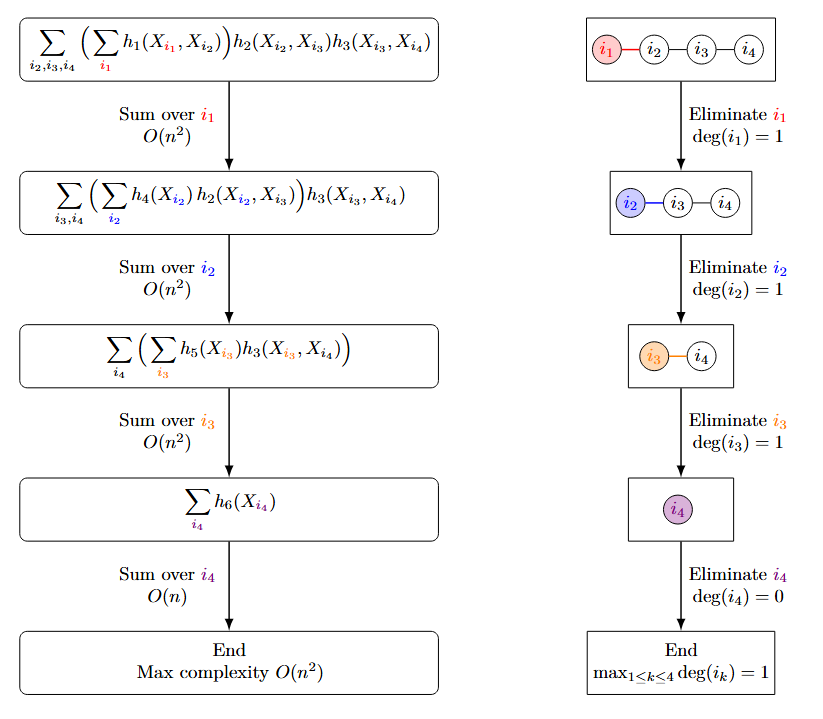
\includegraphics[width=0.8\linewidth]{complexity.jpg}
    \caption*{Procedure of Computing a 4-th order V-statistics}
\end{figure}
\end{frame}


\begin{frame}
\frametitle{Computing V-Statistics with Separable Kernels}
\begin{itemize}
\setlength\itemsep{1.5em}
        \item In general, the computational complexity depends on the summation ordering.
        \item The optimal complexity can be bounded by the treewidth of the corresponding graph $G$, precisely $O(n^{\operatorname{tw}(G)+1})$. 
        \vspace{1.5em}
            \begin{itemize}
            \setlength\itemsep{1.5em}
                \item Finding the optimal ordering is known to be NP-hard. 
                \item In practice, heuristic algorithm such as greedy algorithm is used.  
            \end{itemize}
              % \begin{itemize}
              %     % \item The summation ordering corresponds to an optimal vertex elimination ordering in the graph.
              %     \item The complexity is $O(n^{\operatorname{tw}(G)+1})$.
              %     % \item The summation ordering is orgonized as permutation of the indices.
              % \end{itemize}
\end{itemize}
    
\end{frame}

\begin{frame}
    \frametitle{Computing V-Statistics with Separable Kernels}
    For {\bf Question 2 (Computation Techniques)}:
    \begin{itemize}
        \item Can use \texttt{Einsum} to compute the V-statistic efficiently.
              \begin{itemize}
                  \item Implemented in many libraries such as \numpy\ and \torch.
                  \item Can call \numpyeinsum{} or \torcheinsum{} in practice.
                  \item \torch{} provides parallel computing and GPU acceleration.
              \end{itemize}
        \pause
        \item Also take the above V-statistic as an example.
              \begin{align*}
                  V_{n,4}[h] = \sum_{i_1 = 1}^{n} \sum_{i_2 = 1}^{n} \sum_{i_3 = 1}^{n} \sum_{i_4 = 1}^{n} h_1(X_{i_1}, X_{i_2})h_2(X_{i_2}, X_{i_3})h_3(X_{i_3}, X_{i_4}).
              \end{align*}
        \item Assemble each $h_i$ with samples as a tensor:
              \begin{align*}
                  H_1 = \left( h_1(X_{i_1}, X_{i_2}) \right)_{i_1,i_2=1}^{n}, \\
                  H_2 = \left( h_2(X_{i_2}, X_{i_3}) \right)_{i_2,i_3=1}^{n}, \\
                  H_3 = \left( h_3(X_{i_3}, X_{i_4}) \right)_{i_3,i_4=1}^{n}.
              \end{align*}
        \item $V_{n,4}[h]$ can be computed via
              \begin{align*}
                  V_{n,4}[h] = \texttt{Einsum}(\mathrm{"ab,bc,cd\to"}, H_1, H_2, H_3).
              \end{align*}
    \end{itemize}
\end{frame}

\begin{frame}
    \frametitle{Computing V-Statistics with Separable Kernels}
    \begin{itemize}
    \setlength\itemsep{1.5em}
        \item For \texttt{Einsum}, \numpy{} and \opteinsum{} find an efficient summation ordering by minimizing the FLOPs, using
        \vspace{1.5em}
              \begin{itemize}
            \setlength\itemsep{1.5em}
                  \item greedy algorithms,
                  \item dynamic programming, 
                  \item exhaustive search .etc.
                  % \item The summation ordering is orgonized as pairs of tensors
              \end{itemize}
        \item The complexity is given by accurate counting of FLOPs.
        \item Finding the optimal summation ordering is NP-hard in general.
              \begin{itemize}
                  \item Computing the treewidth of a graph is known to be NP-hard.
              \end{itemize}
    \end{itemize}
\end{frame}


\begin{frame}
    \frametitle{Computing U-Statistics with Separable Kernels}
    \begin{itemize}
        \item The trick can't be applied directly, because the indices are not independent.
              \begin{itemize}
                  \item Any two indices must be different.
              \end{itemize}
        \item Our strategy is to decompose U-statistics to V-statistics using the \textbf{M\"obius inversion} technique.
              \begin{mylemma}[Decomposition of U-statistics to V-statistics]
                  \label{lem:decomp_u_to_v}
                  Let $\bbX$ be a non-empty set and $h: \bbX^{m} \rightarrow \bbR$ be a kernel function. Then for any $\bm{X} \in \bbX^n: n \geq m$,
                  \begin{align*}
                      \ustat(h,\bm{X}) = \sum_{\sPi \in \partitionp{m}}
                      \mu_\sPi \vstat[\sPi](h, \bm{X}),
                  \end{align*}
                  where
                  \begin{align*}
                      \mu_\sPi = (-1)^{(m-|\sPi|)} \prod_{C \in \sPi} (|C| - 1)!.
                  \end{align*}
              \end{mylemma}
        % \item Thus the complexity also is reduced and can be computed via \texttt{Einsum} as well.
    \end{itemize}
\end{frame}


\begin{frame}
    \frametitle{Computing U-Statistics with Separable Kernels}
    \begin{itemize}
        \item For U-statistic similar to the example in computing V-statistics, it takes the form
              \begin{align*}
                  U_{n,4}[h] = \sum_{i_1 \neq i_2 \neq i_3 \neq i_4} h_1(X_{i_1}, X_{i_2}) h_2(X_{i_2}, X_{i_3}) h_3(X_{i_3}, X_{i_4}).
              \end{align*}
        \item It can be decomposed to a combiation of $15$ lower order V-statistics 
              \begin{align*}
                  U_{n,4}[h] = & \sum_{i_1,i_2,i_3,i_4=1}^{n} h\underbrace{(X_{i_1}, X_{i_2}, X_{i_3}, X_{i_4})}_{{\color{red} \text{no restriction}\, \pi = \{1,2,3,4\}}} \quad {\color{red} 4\text{ order}} \\
                    {\color{red} 3\text{ order}}& -\sum_{i_1,i_2,i_3 = 1}^{n} h(\underbrace{X_{i_1}, X_{i_1}, X_{i_3}, X_{i_4}}_{{\color{red} i_1=i_2 \, \pi=\{\{1,2\},3,4\}}}) - \sum_{i_1,i_2,i_4 =1}^{n} h(\underbrace{X_{i_1}, X_{i_2}, X_{i_1}, X_{i_4}}_{{\color{red} i_1=i_3 \, \pi = \{\{1,3\},2,4\}}}) - \cdots \\
                    {\color{red} 2\text{ order}}& +            \sum_{i_1,i_3 = 1}^{n} h(\underbrace{X_{i_1}, X_{i_1}, X_{i_3}, X_{i_3}}_{{\color{red} i_1=i_2,i_3=i_4}}) + \sum_{i_1,i_2 = 1}^{n} h(\underbrace{X_{1}, X_{i_2}, X_{i_1}, X_{i_2}}_{{\color{red} i_1=i_3,i_2=i_4}}) + \cdots \\
                    \color{red} 1\text{ order}& +6 \sum_{i_1= 1}^{n} h(\underbrace{X_{i_1}, X_{i_1}, X_{i_1}, X_{i_1}}_{{\color{red} i_1=i_2=i_3=i_4}})
              \end{align*}
    \end{itemize}
\end{frame}

\begin{frame}
\frametitle{Computing U-Statistics with Separable Kernels}
\begin{itemize}
    \item The complexity is reduced to $O(n^3)$, compared with naively $O(n^4)$, 
    \begin{itemize}
        \item and can be computed via \texttt{Einsum} as well.
    \end{itemize}
    \item For higher order U-statistics like the above,  
    \begin{align*}
        U_{n,m}[h] = \sum_{i_1 \neq \cdots \neq i_m} h_1(X_{i_1}, X_{i_2}) h_2(X_{i_2},X_{i_3}) \cdots h_{m-1}(X_{m-1}, X_m), 
    \end{align*}
    the computational complexity is
\end{itemize}
\vspace{1.5em}
\begin{equation*}
\begin{array}{c|c}
\hline
\textbf{Order ($m$)} & \textbf{Complexity} \\
\hline
2, 3 & O(n^2) \\
4, 5, 6, 7 & O(n^3) \\
 8, 9, 10 & O(n^4) \\
\hline
\end{array}
\end{equation*}
\end{frame}


\begin{frame}
\frametitle{Computing U-Statistics with Separable Kernels}
\begin{itemize}
    \item Bell number: the number of V-statistics to compute a $m$-th order U-statistics. 
    \begin{itemize}
        \item is known to grow super-exponentially w.r.t. order $m$. 
    \end{itemize}
    \item We develop a {\bf cancellation trick} to reduce the number of terms. 
    \item For HOIF-type U-statistics, 
\end{itemize}
\begin{table}[h!]
\centering
\begin{tabular}{cccc}
\toprule
\textbf{Order ($m$)} & \makecell{\textbf{V-stat terms} \\ \textbf{(Bell number)}} & \makecell{\textbf{V-stat terms} \\ \textbf{(cancellation)}} & \textbf{Ratio} \\
\midrule
3  & 5       & 2       & 0.4 \\
4  & 15      & 5       & 0.333 \\
5  & 52      & 15      & 0.288 \\
6  & 203     & 52      & 0.256 \\
7  & 877     & 203     & 0.231 \\
8  & 4140    & 877     & 0.212 \\
9  & 21147   & 4140    & 0.196 \\
10 & 115975  & 21147   & 0.182 \\
11 & 678570  & 115975  & 0.171 \\
12 & 4213597 & 678570  & 0.161 \\
\bottomrule
\end{tabular}
\end{table}   
\end{frame}


\section{Our New Package \package{} for Computing U-Statistics}
\begin{frame}
    \frametitle{Outline}
    \tableofcontents[currentsection, sectionstyle=show/shaded, subsectionstyle=show/shaded/shaded]
\end{frame}
\begin{frame}
    \frametitle{Our New Package \package{} for Computing U-Statistics}
    \begin{itemize}
        \item Github Link:  \url{https://github.com/Amedar-Asterisk/U-Statistics-python}
        \item Some instructions can also be found in the \texttt{README.md} file of the repository.
    \end{itemize}
    \begin{figure}
        \centering
        
\includegraphics[width=0.5\linewidth]{github_QR.png}
        \caption*{QR code}
    \end{figure}
\end{frame}

\begin{frame}
    \frametitle{Our New Package \package{} for Computing U-Statistics}
    \begin{itemize}
        \item It was also available on \texttt{PyPI}: \url{https://pypi.org/project/u-stats/},
        \item and can be installed via
              \begin{align*}
                  \texttt{pip install u-stats}
              \end{align*}
    \end{itemize}
    \begin{figure}
        \centering
        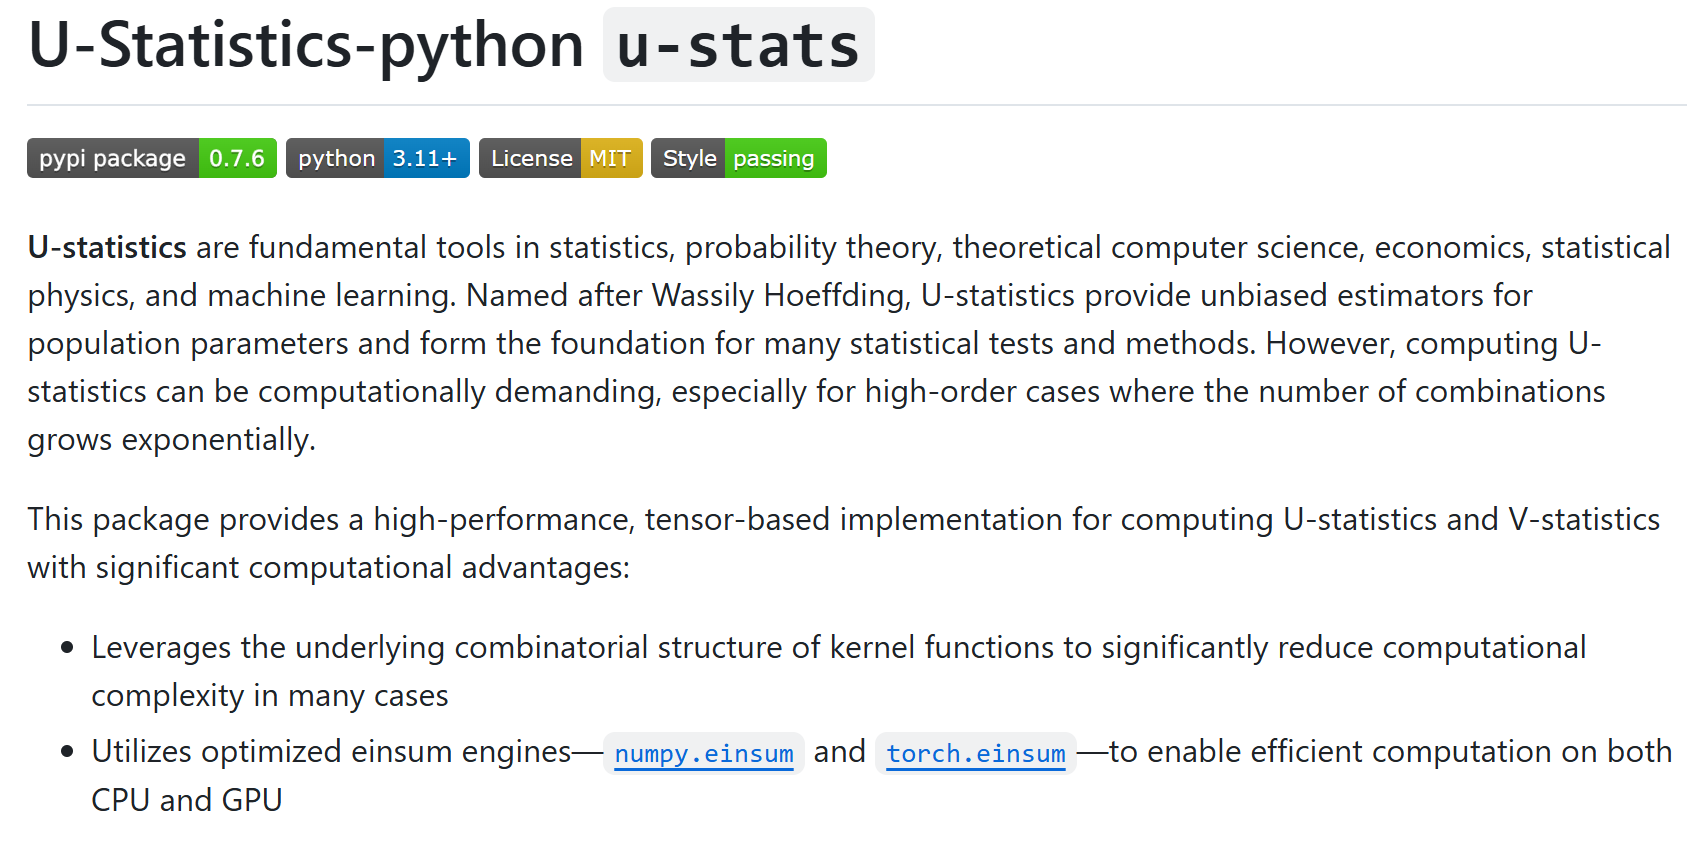
\includegraphics[width=\linewidth]{github.png}
    \end{figure}
\end{frame}

\section{Applications}
\begin{frame}
    \frametitle{Outline}
    \tableofcontents[currentsection, sectionstyle=show/shaded, subsectionstyle=show/shaded/shaded]
\end{frame}
\begin{frame}
    \frametitle{Application 1: Higher-Order Influence Functions}
    \begin{itemize}
        \item HOIFs involve computing a class of U-statistics like
              \begin{align*}
                  \bbU_{n,m}(h^{(m)}) = \sum_{i_1 \neq i_2 \neq \cdots \neq i_m} h^{(m)}_1(X_{i_1}, X_{i_2}) h^{(m)}_2(X_{i_2}, X_{i_3}) \cdots h^{(m)}_{m-1}(X_{i_{m-1}}, X_{i_m}).
              \end{align*}
        \item We test \package{} on computing HOIFs on platforms both in CPU and GPU (with \torch).
        \item For CPU
              \begin{table}[htbp]
                  \centering
                  \caption{Average runtime (in seconds) using CPU parallel computation. Experiments were conducted on Intel Xeon ICX Platinum 8358 CPUs (2.6GHz, 64 total cores) with 512 GB of memory, evaluated across varying sample sizes and orders of HOIF-type U-statistics.}
                  \label{tab:HOIF_CPU}
                  \begin{tabular}{cccccc}
                      \toprule
                      $\bm{m} \backslash \bm{n}$ & \textbf{1000} & \textbf{2000} & \textbf{4000} & \textbf{8000} & \textbf{10000} \\
                      \midrule
                      2                          & 0.64          & 0.00141       & 0.01298       & 0.03174       & 0.04746        \\
                      3                          & 0.00396       & 0.01518       & 0.07392       & 0.26849       & 0.45976        \\
                      4                          & 0.02321       & 0.07313       & 0.32765       & 2.09545       & 2.36766        \\
                      5                          & 0.09853       & 0.36239       & 1.71419       & 9.11349       & 14.21350       \\
                      6                          & 0.38878       & 1.47719       & 7.44444       & 40.22143      & 58.85063       \\
                      7                          & 1.91677       & 6.75947       & 34.08805      & 195.31414     & 290.54295      \\
                      \bottomrule
                  \end{tabular}
              \end{table}
    \end{itemize}
\end{frame}

\begin{frame}
    \frametitle{Application 1: Higher-Order Influence Functions}
    \begin{itemize}
        \item For GPU
              \begin{table}[htbp]
                  \centering
                  \caption{Average runtime (in seconds) using a single GPU (NVIDIA RTX 4090, 24GB) with parallel computation, across varying sample sizes and orders of HOIF-type U-statistics.}
                  \label{tab:HOIF_GPU}
                  \begin{tabular}{cccccc}
                      \toprule
                      $\bm{m} \backslash \bm{n}$ & \textbf{1000} & \textbf{2000} & \textbf{4000} & \textbf{8000} & \textbf{10000} \\
                      \midrule
                      2                          & 0.00184       & 0.00151       & 0.00155       & 0.00238       & 0.00339        \\
                      3                          & 0.00172       & 0.00147       & 0.00193       & 0.00577       & 0.00745        \\
                      4                          & 0.00305       & 0.00353       & 0.00707       & 0.03612       & 0.06245        \\
                      5                          & 0.00835       & 0.01089       & 0.03456       & 0.19807       & 0.36160        \\
                      6                          & 0.02608       & 0.03906       & 0.16981       & 1.12072       & 2.13328        \\
                      7                          & 0.12031       & 0.19132       & 0.91884       & 6.45225       & 12.21350       \\
                      \bottomrule
                  \end{tabular}
              \end{table}
    \end{itemize}
\end{frame}

\begin{frame}
    \frametitle{Application 2: Distance Covariance}
    \begin{itemize}
        \item We also test our algorithm on computing $\mathsf{dCov}^2$
              \begin{align*}
                  \mathsf{dCov}^2(X, Y) = \frac{(n-4)!}{n!} \sum_{i \neq j \neq q \neq r}
                  a_{i,j}b_{q,r} + a_{i,j}b_{i,j} - a_{i,j}b_{i,q} - a_{i,j}b_{j,r}
              \end{align*}
        \item We compare the performance with \cite{shao2025u}
              \begin{itemize}
                  \item They use a randomized incomplete algorithm to compute $\mathsf{dCov}^2$.
                  \item $\alpha$ is a tuning parameter to control the degree of completeness.
                  \item Randomized algorithm of $\alpha$ takes $O(n^{\alpha})$ time.
              \end{itemize}

    \end{itemize}
    \begin{table}[htbp]
        \centering
        \caption{
            Runtime comparison of
            Experiments were run on CPU with 8 cores.
        }
        \label{tab:dcov}
        \begin{tabular}{cc|cccc}
            \toprule
            \makecell{\textbf{\texttt{u-stats}}                     \\ \textbf{No Parallel} } &
            \makecell{\textbf{\texttt{u-stats}}                     \\ \textbf{Parallel} } &
            \makecell{\textbf{Randomized}                           \\ \textbf{$\alpha = 1.5$}} &
            \makecell{\textbf{Randomized}                           \\ \textbf{$\alpha = 2.0$}} &  \makecell{\textbf{Randomized} \\ \textbf{$\alpha = 2.5$}} &
            \makecell{\textbf{Complete}}                            \\
            \midrule
            2.3701 & 0.1894 & 0.3860 & 4.8164 & 56.4892 & 3787.8360 \\
            \bottomrule
        \end{tabular}
    \end{table}
\end{frame}

\begin{frame}
    \frametitle{Application 3: Motif Counts}
    \begin{itemize}
    \setlength\itemsep{1.5em}
        \item We compare the performance of our \package{} with  \igraph{}.
        \item On Erdős-Rényi graphs $G(n, p)$:
            \begin{itemize}
            \setlength\itemsep{1.5em}
                \item $n$ is the number of vertices. 
                \item $p$ is the probability of edge existence. 
                \item CPU parallel with 64 cores via \torch{} for \package{}.
                \item Count all types of 3-node or 4-node motifs. 
            \end{itemize}
    \end{itemize}
\end{frame}

\begin{frame}
    \frametitle{Application 3: Motif Counts}
    \begin{itemize}
        \item For the 3-node motifs,
    \end{itemize}
    \begin{table}
        \centering
        \caption{
            Runtime comparison of exact all $3$-node motif counts using \texttt{u-stats} and \texttt{igraph} on Erdős-Rényi graphs $G(n, p)$ with $n = 5623$.
            Experiments were run on Intel Xeon ICX Platinum 8358 CPUs (2.6GHz, 64 total cores) with 512 GB of memory.
            "Speedup ratio" compares \texttt{igraph} to our parallel method; "single core speedup" assumes single-core execution.
        }
        \label{tab:motif_counts_3}
        \begin{tabular}{ccccc}
            \toprule
            \makecell{\textbf{Edge}                      \\ \textbf{Prob.} $p$} & \makecell{\textbf{\texttt{u-stats}} \\ \textbf{Time (s)}} & \makecell{\textbf{\texttt{igraph}} \\ \textbf{Time (s)}} &\makecell{\textbf{Speedup} \\ \textbf{Ratio}} &  \makecell{\textbf{Single-Core} \\ \textbf{Speedup}} \\
            \midrule
            0.001 & 0.617 & 0.025    & 0.040    & 0.001  \\
            0.005 & 0.649 & 0.353    & 0.544    & 0.008  \\
            0.010 & 0.692 & 1.795    & 2.595    & 0.041  \\
            0.020 & 0.783 & 10.594   & 13.529   & 0.211  \\
            0.050 & 1.038 & 136.272  & 131.288  & 2.051  \\
            0.080 & 1.298 & 514.702  & 396.415  & 6.194  \\
            0.100 & 1.453 & 960.299  & 660.690  & 10.323 \\
            0.150 & 1.864 & 3003.490 & 1611.389 & 25.178 \\
            0.200 & 2.275 & 6725.515 & 2955.656 & 46.182 \\
            \bottomrule
        \end{tabular}
    \end{table}
\end{frame}

\begin{frame}
    \frametitle{Application 3: Motif Counts}

    \begin{itemize}
        \item For the 4-node motifs,
    \end{itemize}
    \begin{table}
        \centering
        \caption{
            Runtime comparison of exact all $4$-node motif counts using \texttt{u-stats} and \texttt{igraph} on Erdős-Rényi graphs $G(n, p)$ with $n = 2000$.
            Experiments were run on Intel Xeon ICX Platinum 8358 CPUs (2.6GHz, 64 total cores) with 512 GB of memory.
            "Speedup ratio" compares \texttt{igraph} to our parallel method; "single core speedup" assumes single-core execution.
        }
        \label{tab:motif_counts_4}
        \begin{tabular}{ccccc}
            \toprule
            \makecell{\textbf{Edge}                       \\ \textbf{Prob.} $p$} & \makecell{\textbf{\texttt{u-stats}} \\ \textbf{Time (s)}} & \makecell{\textbf{\texttt{igraph}} \\ \textbf{Time (s)}} &\makecell{\textbf{Speedup} \\ \textbf{Ratio}} &  \makecell{\textbf{Single-Core} \\ \textbf{Speedup}} \\
            \midrule
            0.001 & 70.959 & 0.004     & 0.      & 0.     \\
            0.005 & 71.947 & 0.168     & 0.002   & 0.     \\
            0.010 & 68.463 & 1.453     & 0.021   & 0.     \\
            0.020 & 65.634 & 15.573    & 0.237   & 0.004  \\
            0.050 & 65.786 & 394.532   & 5.997   & 0.094  \\
            0.080 & 66.866 & 2371.373  & 35.465  & 0.554  \\
            0.100 & 68.219 & 5396.057  & 79.099  & 1.236  \\
            0.150 & 65.969 & 23003.041 & 348.692 & 5.448  \\
            0.200 & 65.259 & 61796.760 & 946.940 & 14.796 \\
            \bottomrule
        \end{tabular}
    \end{table}
\end{frame}

\section{Limitations and Future Work}
\begin{frame}
    \frametitle{Outline}
    \tableofcontents[currentsection, sectionstyle=show/shaded, subsectionstyle=show/shaded/shaded]
\end{frame}
\begin{frame}
    \frametitle{Limitations and Future Work}
    \begin{itemize}
    \setlength\itemsep{1.5em}
        \item Limitations:
              \begin{itemize}
              \setlength\itemsep{1.5em}
                  \item Memory usage is high: for HOIFs, it's not available for sample size larger than $2000$ and order larger than $8$ -- Hybrid between for-loop \& Einsum (or we can wait for better GPUs)?

                  \item How to combine our techniques with randomized incomplete U-statistics \citep{chen2019randomized, shao2025u}?
              \end{itemize}
        \item Future work:
              \begin{itemize}
                  \item Interface for \texttt{R}.
                  \item Non-scalar-valued U-statistics.
              \end{itemize}
    \end{itemize}
\end{frame}

\section*{References}
\begin{frame}
    \frametitle{References}
    \bibliography{Master}
\end{frame}
\end{document}